\documentclass{beamer}
\usepackage[utf8]{inputenc}

\usetheme{Madrid}
\usecolortheme{default}
\usepackage{amsmath,amssymb,amsfonts,amsthm}
\usepackage{txfonts}
\usepackage{tkz-euclide}
\usepackage{listings}
\usepackage{adjustbox}
\usepackage{array}
\usepackage{tabularx}
\usepackage{gvv}
\usepackage{lmodern}
\usepackage{circuitikz}
\usepackage{tikz}
\usepackage{graphicx}
\usepackage{multicol}

\setbeamertemplate{page number in head/foot}[totalframenumber]

\usepackage{tcolorbox}
\tcbuselibrary{minted,breakable,xparse,skins}



\definecolor{bg}{gray}{0.95}
\DeclareTCBListing{mintedbox}{O{}m!O{}}{%
  breakable=true,
  listing engine=minted,
  listing only,
  minted language=#2,
  minted style=default,
  minted options={%
    linenos,
    gobble=0,
    breaklines=true,
    breakafter=,,
    fontsize=\small,
    numbersep=8pt,
    #1},
  boxsep=0pt,
  left skip=0pt,
  right skip=0pt,
  left=25pt,
  right=0pt,
  top=3pt,
  bottom=3pt,
  arc=5pt,
  leftrule=0pt,
  rightrule=0pt,
  bottomrule=2pt,
  toprule=2pt,
  colback=bg,
  colframe=orange!70,
  enhanced,
  overlay={%
    \begin{tcbclipinterior}
    \fill[orange!20!white] (frame.south west) rectangle ([xshift=20pt]frame.north west);
    \end{tcbclipinterior}},
  #3,
}
\lstset{
    language=C,
    basicstyle=\ttfamily\small,
    keywordstyle=\color{blue},
    stringstyle=\color{orange},
    commentstyle=\color{green!60!black},
    numbers=left,
    numberstyle=\tiny\color{gray},
    breaklines=true,
    showstringspaces=false,
}


\title 
{1.3.8}
\date{}

\author
{SAMYAK GONDANE - AI25BTECH11029}


\begin{document}

\frame{\titlepage}
\begin{frame}{Question}
ABCD is a rectangle formed by the points \textbf{A}($-1,-1$), \textbf{B}($-1,6$), \textbf{C}($3,6$) and \textbf{D}($3,-1$). \textbf{P}, \textbf{Q}, \textbf{R} and \textbf{S} are mid-points of sides AB, BC, CD and DA respectively. Show that diagonals of the quadrilateral PQRS bisect each other.
\end{frame}



\vspace{0.5cm}

\begin{frame}{Solution}
    \textbf{Step 1:} Represent Points as Column Vectors

    Let’s define the points as column vectors:\\
    \vspace{0.3cm}
    $\begin{aligned}
    A = \myvec{-1 \\ -1}, \quad 
    B = \myvec{-1 \\ 6}, \quad 
    C = \myvec{3 \\ 6}, \quad 
    D = \myvec{3 \\ 1} 
    \end{aligned}$
    \begin{figure}[H]
        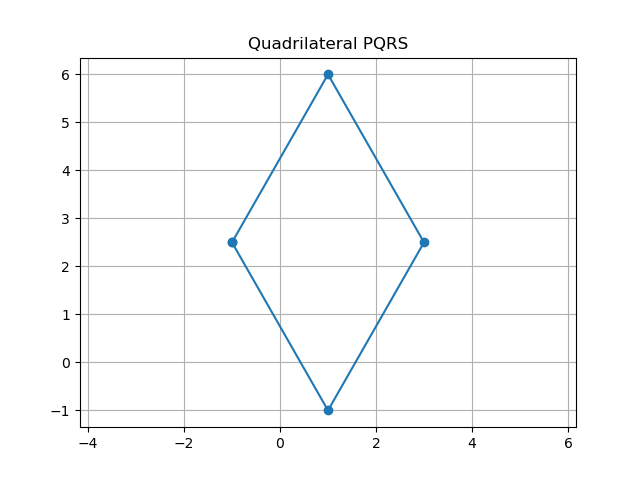
\includegraphics[width=0.5\linewidth]{./figs/Figure_1.png}
        \caption{}
        \label{fig:fig1}
    \end{figure}
\end{frame}


\begin{frame}{Solution}
\textbf{Step 2:} Midpoints as Matrix Expressions

So,
\begin{align}
P = \frac{1}{2}(A + B) = \frac{1}{2} \myvec{-1 + (-1) \\ -1 + 6} = \myvec{-1 \\ 2.5}\\
Q = \frac{1}{2}(B + C) = \frac{1}{2} \myvec{-1 + 3 \\ 6 + 6} = \myvec{1 \\ 6}\\
R = \frac{1}{2}(C + D) = \frac{1}{2} \myvec{3 + 3 \\ 6 + 1} = \myvec{3 \\ 3.5}\\
S = \frac{1}{2}(D + A) = \frac{1}{2} \myvec{3 + (-1) \\ 1 + (-1)} = \myvec{1 \\ 0}
\end{align}
\end{frame}



\begin{frame}{Solution}
\textbf{Step 3:} Diagonals PR and QS

Diagonal PR:

\text{Midpoint}_{PR} = \frac{1}{2}(P + R) = \frac{1}{2} \left( \myvec{-1 \\ 2.5} + \myvec{3 \\ 3.5} \right) = \myvec{1 \\ 3}

\vspace{0.3cm}

Diagonal QS:

\text{Midpoint}_{QS} = \frac{1}{2}(Q + S) = \frac{1}{2} \left( \myvec{1 \\ 6} + \myvec{1 \\ 0} \right) = \myvec{1 \\ 3}
\end{frame}

\begin{frame}{Conclusion}
Since both diagonals PR and QS have the same midpoint \myvec{1 \\ 3} they bisect each other.

\end{frame}




\end{document}
